\documentclass{article}
\usepackage{tikz}
\title{Homework 9}
\author{John Carlyle}

\begin{document}
\maketitle

\begin{description}
\item[4.28.]
  Draw an NFA for the following grammar:\\
  $S \rightarrow abA ~|~ bB ~|~ aba\\
  A \rightarrow b ~|~ aB ~|~ bA\\
  B \rightarrow aB ~|~ aA$

  \begin{center}
    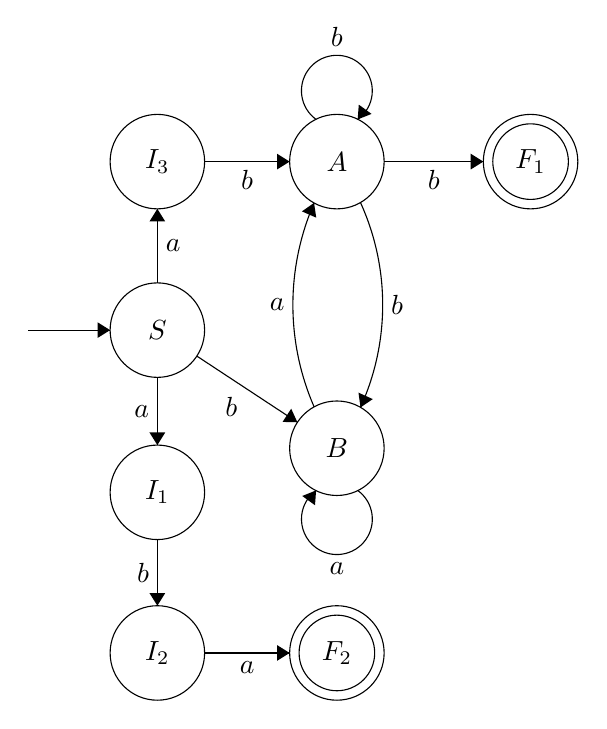
\begin{tikzpicture}[scale=0.2]
      \tikzstyle{every node}+=[inner sep=0pt]
      \draw [black] (17.9,-26.4) circle (3);
      \draw (17.9,-26.4) node {$S$};
      \draw [black] (17.9,-36.7) circle (3);
      \draw (17.9,-36.7) node {$I_1$};
      \draw [black] (17.9,-46.9) circle (3);
      \draw (17.9,-46.9) node {$I_2$};
      \draw [black] (29.3,-46.9) circle (3);
      \draw (29.3,-46.9) node {$F_2$};
      \draw [black] (29.3,-46.9) circle (2.4);
      \draw [black] (29.3,-33.9) circle (3);
      \draw (29.3,-33.9) node {$B$};
      \draw [black] (29.3,-15.7) circle (3);
      \draw (29.3,-15.7) node {$A$};
      \draw [black] (41.6,-15.7) circle (3);
      \draw (41.6,-15.7) node {$F_1$};
      \draw [black] (41.6,-15.7) circle (2.4);
      \draw [black] (17.9,-15.7) circle (3);
      \draw (17.9,-15.7) node {$I_3$};
      \draw [black] (9.7,-26.4) -- (14.9,-26.4);
      \fill [black] (14.9,-26.4) -- (14.1,-25.9) -- (14.1,-26.9);
      \draw [black] (17.9,-29.4) -- (17.9,-33.7);
      \fill [black] (17.9,-33.7) -- (18.4,-32.9) -- (17.4,-32.9);
      \draw (17.4,-31.55) node [left] {$a$};
      \draw [black] (17.9,-39.7) -- (17.9,-43.9);
      \fill [black] (17.9,-43.9) -- (18.4,-43.1) -- (17.4,-43.1);
      \draw (17.4,-41.8) node [left] {$b$};
      \draw [black] (20.9,-46.9) -- (26.3,-46.9);
      \fill [black] (26.3,-46.9) -- (25.5,-46.4) -- (25.5,-47.4);
      \draw (23.6,-47.4) node [below] {$a$};
      \draw [black] (20.41,-28.05) -- (26.79,-32.25);
      \fill [black] (26.79,-32.25) -- (26.4,-31.39) -- (25.85,-32.23);
      \draw (22.6,-30.65) node [below] {$b$};
      \draw [black] (30.623,-36.58) arc (54:-234:2.25);
      \draw (29.3,-41.15) node [below] {$a$};
      \fill [black] (27.98,-36.58) -- (27.1,-36.93) -- (27.91,-37.52);
      \draw [black] (27.977,-13.02) arc (234:-54:2.25);
      \draw (29.3,-8.45) node [above] {$b$};
      \fill [black] (30.62,-13.02) -- (31.5,-12.67) -- (30.69,-12.08);
      \draw [black] (32.3,-15.7) -- (38.6,-15.7);
      \fill [black] (38.6,-15.7) -- (37.8,-15.2) -- (37.8,-16.2);
      \draw (35.45,-16.2) node [below] {$b$};
      \draw [black] (30.796,-18.295) arc (24.49129:-24.49129:15.692);
      \fill [black] (30.8,-31.31) -- (31.58,-30.78) -- (30.67,-30.37);
      \draw (32.71,-24.8) node [right] {$b$};
      \draw [black] (27.855,-31.276) arc (-156.45746:-203.54254:16.213);
      \fill [black] (27.85,-18.32) -- (27.08,-18.86) -- (27.99,-19.26);
      \draw (26.01,-24.8) node [left] {$a$};
      \draw [black] (17.9,-23.4) -- (17.9,-18.7);
      \fill [black] (17.9,-18.7) -- (17.4,-19.5) -- (18.4,-19.5);
      \draw (18.4,-21.05) node [right] {$a$};
      \draw [black] (20.9,-15.7) -- (26.3,-15.7);
      \fill [black] (26.3,-15.7) -- (25.5,-15.2) -- (25.5,-16.2);
      \draw (23.6,-16.2) node [below] {$b$};
    \end{tikzpicture}
  \end{center}

\item[4.29.]\hfill\\
  \begin{description}
    \item[d.]
      $S \rightarrow AB ~~ A \rightarrow aAa ~|~ bAb ~|~ a ~|~ b ~~ B \rightarrow aB ~|~ bB ~|~ \lambda$\\
      Odd length palindrones are being generated. A regular grammar that generates odd length palindrones is:\\
      $S \rightarrow aS ~|~ bS ~|~ aA ~|~ bA\\
      A \rightarrow \lambda$
    \item[e.]
      $S \rightarrow AA ~|~ B ~~ A \rightarrow AAA ~|~ Ab ~|~ bA ~|~ a ~~ B \rightarrow bB ~|~ \lambda$
      Clearly this grammar describes the language with an even number of a's. A regular grammar for this is:\\
      $S \rightarrow aA ~|~ bS ~|~ \lambda\\
      A  \rightarrow aS ~|~ bA$
  \end{description}

\item[55.]
  Let $L \subset \Sigma^*_1$ be a context free language. There must be a CFG to represent this language call it: $G = (V, \Sigma_1, S, P_1)$ s.t. $L = L(G_1)$.
  Let $G_2 = (V, \Sigma_2, S, P_2)$ and let the function $f: \Sigma_1^* \rightarrow \Sigma_2^*$ be homomorphic. Extend $f$ to $g: (\Sigma_1 \cup V)^* \rightarrow (\Sigma_2 \cup V)^*$ where $F(A) = A ~~! \forall A \in V$ 
  Finally $P_2$ is defined as $\forall$ productions $A \rightarrow \alpha \in P_1$, there is a corresponding production $A \rightarrow f(\alpha) \in P_2$ Now we must show that $f(L) = L(G_2)$

  \begin{description}
    \item[$\Rightarrow$]
      if $y \in f(L)$ then $\Rightarrow y \in L(G_2)$
      
      Assume that $y \in f(L)$ then $ \exists x \in L$ s.t. $y = f(x)$. But since $x \in L = L(G_1)$ there is a derivation $S \rightarrow^*_{G_1} x$. Now $g$ can be applied to every derivation in $G_2$ hence $y \in L(G_2)$.

      \item[$\Leftarrow$]
        If $y \in L(G_2)$ then there is a derviation $S \rightarrow^*_{G_2} y$ of the form $A \rightarrow f(x)$ and $x \in L$ therefore $y$ must be an element of $F(L)$.
  \end{description}

\item[5.1]
  \begin{description}
  \item[a.]\hfill\\
    \begin{description}
    \item[String: ab]
      $(q_0, ab, Z_0) \vdash (q_1, b, aZ_0) \vdash (q_2, \lambda, Z_0) \vdash (q_3, \lambda, Z_0)$. Hence ab is accepted.
    \item[String: aab]
      $(q_0, aab, Z_0) \vdash (q_1, ab, aZ_0) \vdash (q_1, b, aaZ_0) \vdash (q_2, \lambda, aZ_0)$. No transition exists for the given inputs, hence the string is not accepted.
    \item[String: abb]
      $(q_0, abb, Z_0) \vdash (q_1, bb, aZ_0) \vdash (q_2, b, Z_0)$. No transition exists for the given inputs, hence the string is not accepted.
    \end{description}
  \item[b.]\hfill\\
    \begin{description}
      \item[String: bacab]
        $(q_0, bacab, Z_0) \vdash (q_0, acab, bZ_0) \vdash (q_0, cab, abZ_0) \vdash (q_1, ab, abZ_0) \vdash (q_1, b, bZ_0) \vdash (q_1, \lambda, Z_0) \vdash (q_2, \lambda, Z_0)$. Hence bacab is accepted.
      \item[String: baca]
        $(q_0, baca, Z_0) \vdash (q_0, aca, bZ_0) \vdash (q_0 ,ca, abZ_0) \vdash (q_1, a, abZ_0) \vdash (q_1, \lambda, bZ_0)$. No transition exists for the given inputs, hence the string is not accepted.
    \end{description}
  \end{description}

\item[4. a.]
  The language of even-length palindromes.\\
  \begin{center}
    \begin{tabular}{|lllll|}
      \hline
      Move & State & Input & Stack & Move(s)\\
      \hline
      1 & $q_0$ & a & $Z_0$ & $(q_0, aZ_0)$\\
      2 & $q_0$ & a & a & $(q_0, aa)$\\
      3 & $q_0$ & a & b & $(q_0, ab)$\\
      4 & $q_0$ & b & $Z_0$ & $(q_0, bZ_0)$\\
      5 & $q_0$ & b & a & $(q_0, ba)$\\
      6 & $q_0$ & b & b & $(q_0, bb)$\\
      7 & $q_0$ & $\lambda$ & $Z_0$ & $(q_1, Z_0)$\\
      8 & $q_0$ & $\lambda$ & a & $(q_1, a)$\\
      9 & $q_0$ & $\lambda$ & b & $(q_1, b)$\\
      10 & $q_1$ & a & a & $(q_1, \lambda)$\\
      11 & $q_1$ & b & b & $(q_1, \lambda)$\\
      12 & $q_1$ & $\lambda$ & $Z_0$ & $(q_2, Z_0)$\\
      \hline
    \end{tabular}
  \end{center}

\item[5.5]
  \begin{description}
  \item[a.]
    The language of all odd-length strings over ${a, b}$ with middle symbol a.
    \begin{center}
      \begin{tabular}{|lllll|}
        \hline
        Move & State & Input & Stack & Move(s)\\
        \hline
        1 & $q_0$ & a & $Z_0$ & $(q_0,aZ_0),(q_1,Z_0)$\\
        2 & $q_0$ & a & a & $(q_0,aa),(q_1,a)$\\
        3 & $q_0$ & a & b & $(q_0,ab),(q_1,b)$\\
        4 & $q_0$ & b & $Z_0$ & $(q_0,bZ_0)$\\
        5 & $q_0$ & b & a & $(q_0,ba)$\\
        6 & $q_0$ & b & b & $(q_0,bb)$\\
        7 & $q_1$ & a & a & $(q_1,\lambda)$\\
        8 & $q_1$ & a & b & $(q_1,\lambda)$\\
        9 & $q_1$ & b & a & $(q_1,\lambda)$\\
        0 & $q_1$ & b & b & $(q_1,\lambda)$\\
        10 & $q_1$ & $\lambda$ & $Z_0$ & $(q_2,Z_0)$\\
        \hline
      \end{tabular}
    \end{center}
    
  \item[b.]
    $\{a^n x | n \ge 0, x \in \{a,b\}^*$ and $|x| \le n\}$.
    \begin{center}
      \begin{tabular}{|l|l|l|l|l|}
        \hline
        Move & State & Input & Stack & Move(s)\\
        \hline
        1 & $q_0$ & $\lambda$ & $Z_0$ & $(q_1,Z_0)$\\
        2 & $q_0$ & a & $Z_0$ & $(q_1,aZ_0)$\\
        3 & $q_0$ & a & a & $(q_0,aa), (q_1,a)$\\
        4 & $q_1$ & a & a & $(q_1,\lambda)$\\
        5 & $q_1$ & b & a & $(q_1,\lambda)$\\
        \hline
      \end{tabular}
    \end{center}
  \item[c.]
    $\{a^i b^j c^k | i,j,k \ge 0$ and $j=i$ or $j = k\}$.
    \begin{center}
      \begin{tabular}{|lllll|}
        \hline
        Move & State & Input & Stack & Move(s)\\
        \hline
        1 & $q_0$ & a & $Z_0$ & $(q_0, aZ_0), (q_0, Z_0)$\\
        2 & $q_0$ & a & a & $(q_0, aa)$\\
        3 & $q_0$ & b & $Z_0$ & $(q_1, bZ_0)$\\
        4 & $q_1$ & b & a & $(q_1, \lambda)$\\
        5 & $q_1$ & b & b & $(q_1, bb)$\\
        6 & $q_1$ & c & $Z_0$ & $(q_3, Z_0)$\\
        7 & $q_1$ & c & $b$ & $(q_2, \lambda)$\\
        8 & $q_2$ & c & $b$ & $(q_2, \lambda)$\\
        9 & $q_2$ & $\lambda$ & $Z_0$ & $(q_3, Z_0)$\\
        10 & $q_3$ & c & $Z_0$ & $(q_3, Z_0)$\\
        11 & $q_3$ & $\lambda$ & $Z_0$ & $(q_4, Z_0)$\\
        \hline
      \end{tabular}
    \end{center}
  \end{description}

\item[5.7]
  All non-palindromes in $\{a,b\}^*$
\end{description}
\end{document}
